\documentclass{beamer}

\mode<presentation>
{
  \usetheme{Berlin}
  \usecolortheme{default}
  \setbeamercovered{transparent}
}

\usepackage[english]{babel}
\usepackage[all]{xy}
\usepackage[latin1]{inputenc}
\usepackage{qtree}
\usepackage{times}
\usepackage{graphics}
\usepackage[T1]{fontenc}


\title[Leren en Beslissen - Sentiment Analisys]
{Sentiment Analysis}

\subtitle{A Probabilistic Approach}

\author[Gieske, Laan, ten Velthuis, Verschoor, Wiggers ] % (optional, use only with lots of authors)
{S.~A.~Gieske \and S.~Laan \and D.~S.~Ten Velthuis \and C.~R.~Verschoor \and A.~J.~Wiggers}

\institute[University of Amsterdam] % (optional, but mostly needed)
{
  Faculty of Science (FNWI) \\
  University of Amsterdam
  }

\AtBeginSection[]
{
  \begin{frame}<beamer>{Outline}  
    \setcounter{tocdepth}{1}
    \tableofcontents[currentsection,currentsubsection]
  \end{frame}
}

\begin{document}

\begin{frame}
  \titlepage
\end{frame}

\begin{frame}{Outline}
  \setcounter{tocdepth}{1}
  \tableofcontents
\end{frame}


\section{The goal}

\begin{frame}{The goal of the project}
\begin{block}{Project Description}
Performing sentiment analysis on messages about the EO
\end{block}
\begin{itemize}
\item Classification Sentiment vs. Non Sentiment
\item Classification Positive vs. Negative
\end{itemize}
\end{frame}

\section{Approach}
\begin{frame}{Approach}
\begin{itemize}
\item Preprocessing of the data
\item Perform machine learning algorithms on data
\item Use best algorithms to classify real time on server
\end{itemize}
\end{frame}
\begin{frame}{Hierarchical Classification}
\begin{figure}[h]
\Tree [.{All messages} {Neutral Messages} [.{Non-Neutral Messages} {Positive Messages} {Negative Messages} ] ]
\end{figure}
\end{frame}


\section{Data Preprocessing}
\begin{frame}<beamer>{Outline}
    \setcounter{tocdepth}{2}
    \tableofcontents[
    currentsubsection, 
    hideothersubsections, 
    sectionstyle=show/hide] 
  \end{frame}
\subsection{Dataset Analysis}
\begin{frame}{Dataset Analysis}
\begin{block}{Dataset messages EO}
10.000 messages, 19 features per message
\end{block}
Ony 3 features used: \\
\begin{itemize}
\item Source
\item Sentiment
\item Message contents
\end{itemize}
\end{frame}


\subsection{Data Cleaning}
\begin{frame}{Data Cleaning}
\begin{itemize}
\item Shorten words, e.g.\ `saaaaaaai' to `saaai'
\item Stemmer
\end{itemize}
\end{frame}

\subsection{Data Reduction}
\begin{frame}{Data Reduction}
\begin{itemize}
\item Only use Twitter messages (83\% of all messages)
\item Remove articles, reference words and prepositions
\item Substitute smileys with words
\item Remove some punctuation marks (e.g.\ not ! ? )
\end{itemize}
\end{frame}

%%%%% CLASSIFICATION
\section{Classification}
\begin{frame}<beamer>{Outline}
    \setcounter{tocdepth}{2}
    \tableofcontents[
    currentsubsection, 
    hideothersubsections, 
    sectionstyle=show/hide] 
  \end{frame}
\begin{frame}{Classification}
\end{frame}

\subsection{Weighted Sum Probability}
\begin{frame}{Weighted Sum Probability}
\begin{itemize}
\item Extract features
\item Assign sentiment probabilities to features
\begin{equation}
P(feature) = \frac{ \sum feature \in C_1}{\sum feature \in C_1\cup C_2}
\end{equation}
\item Assign sentiment probabilities to sentences
\begin{equation}
P(s) = \frac{1}{n} \sum_{f \in s} P(f)
\end{equation}
\end{itemize}
\end{frame}

\begin{frame}{WSP: Neutral vs Non-Neutral}
\centering
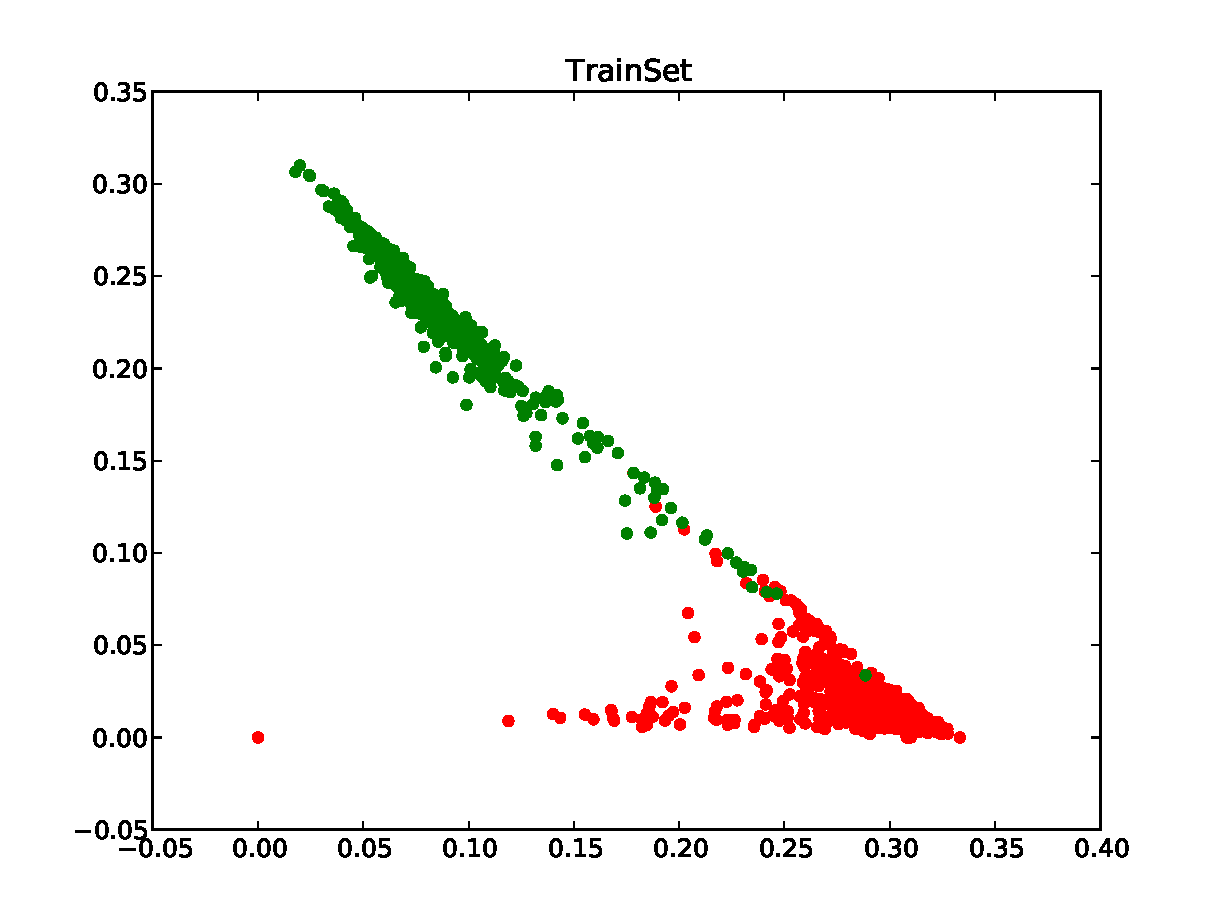
\includegraphics[scale=0.25]{NeuNonNeuScatter1.pdf}
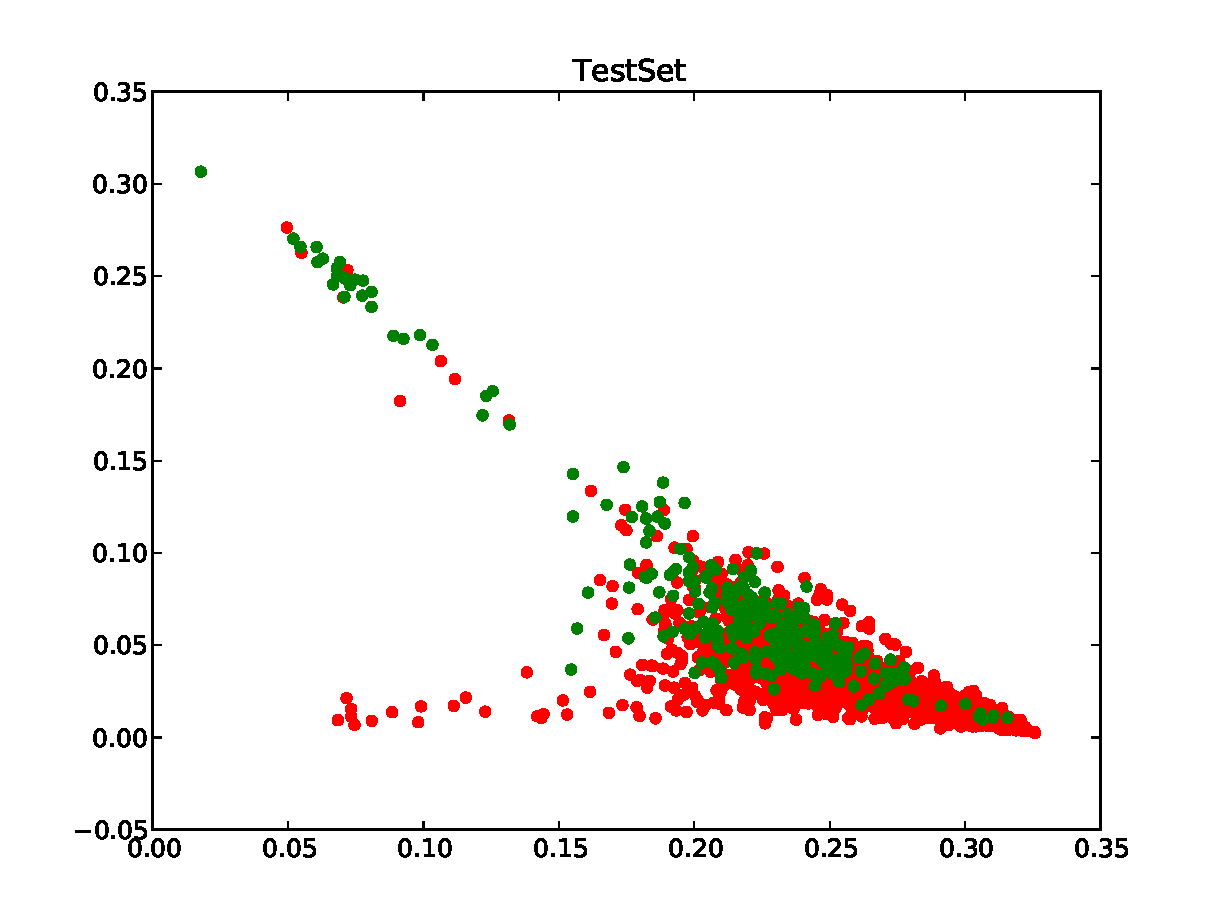
\includegraphics[scale=0.25]{NeuNonNeuScatter2.pdf}
\end{frame}

\begin{frame}{WSP:Positive vs Negative}
\centering
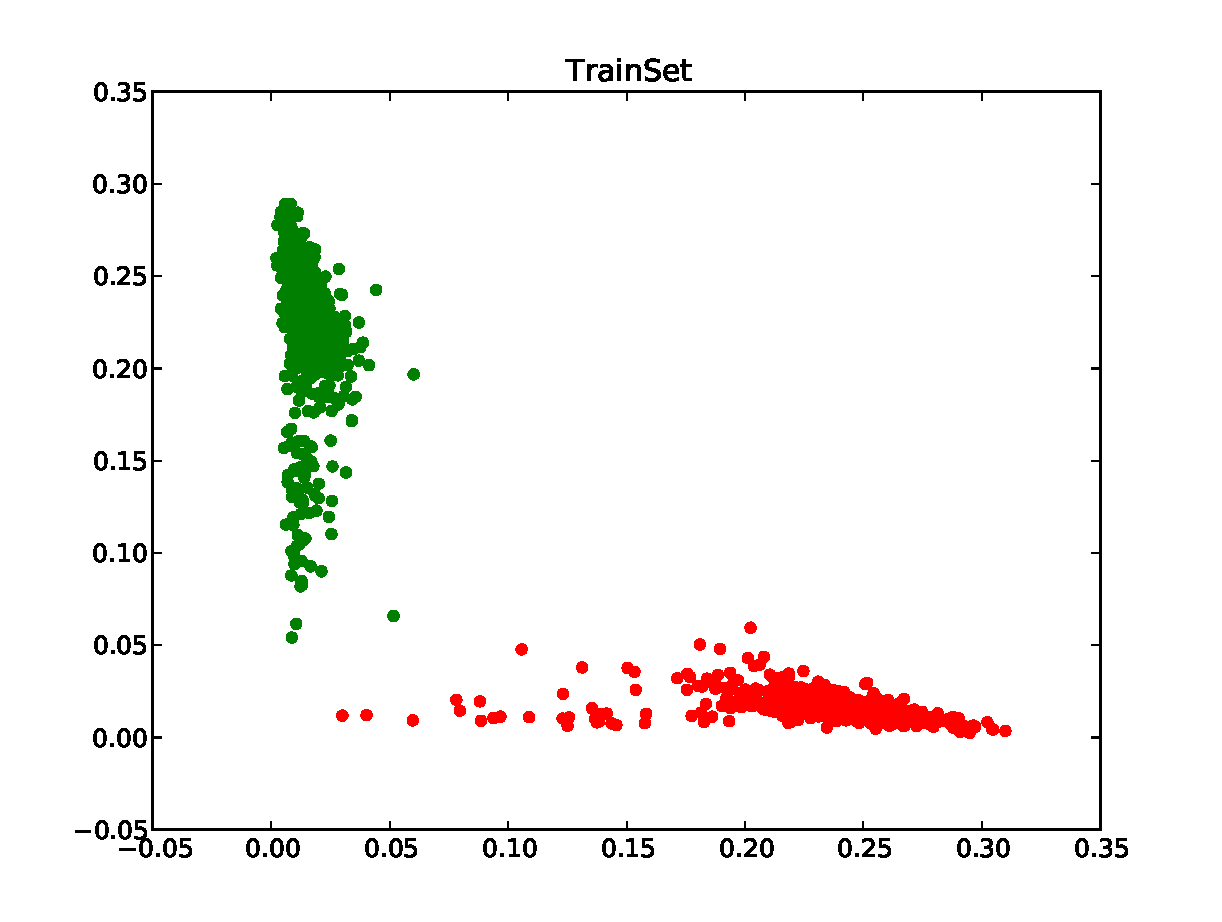
\includegraphics[scale=0.25]{PosNegScatter1.pdf}
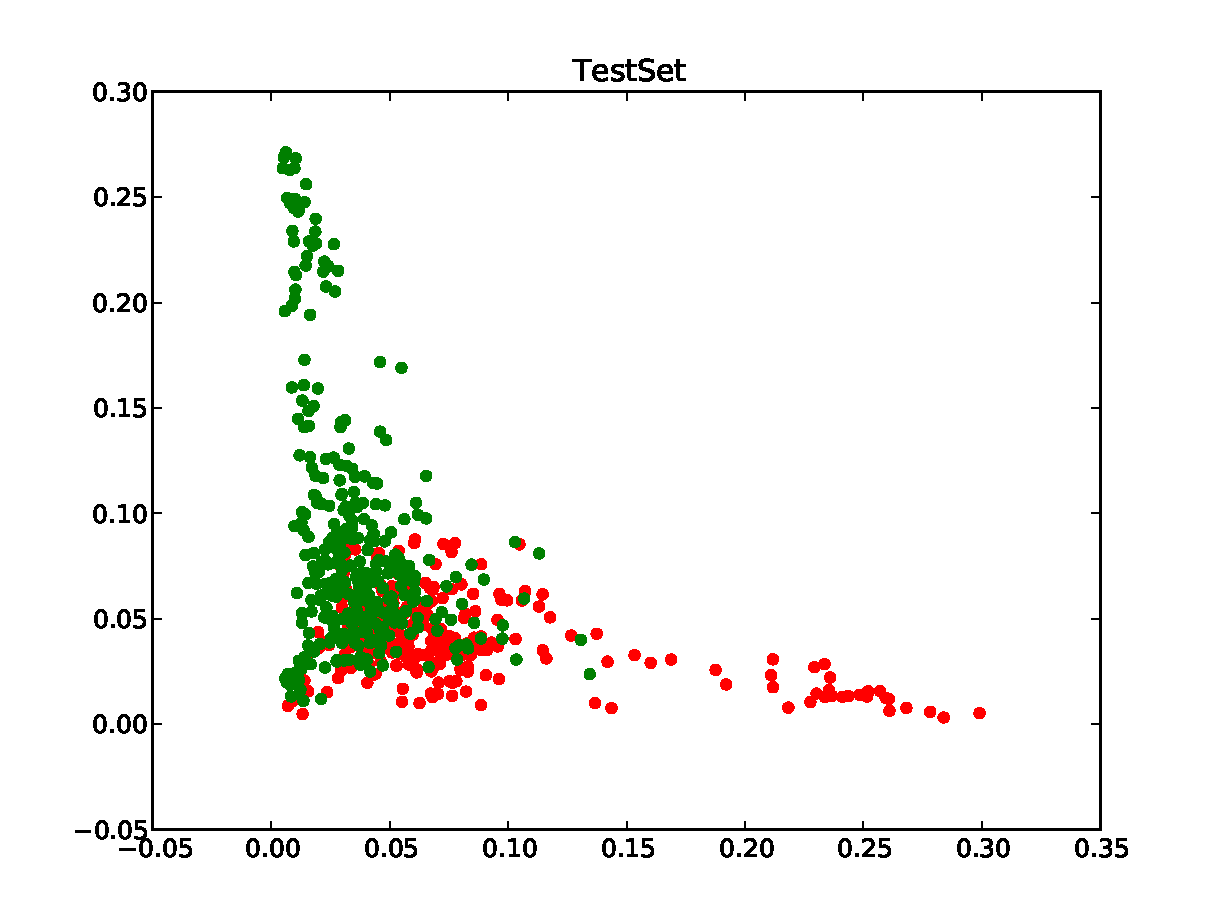
\includegraphics[scale=0.25]{PosNegScatter2.pdf}
\end{frame}

\subsection{Perceptron}
\begin{frame}{Perceptron}
\begin{block}{Algorithm}
Train linear treshold
\end{block}
\begin{description}
\item[Input]: Sentence probabilities, sentence values
\item[Output]: Treshold
\end{description}
\end{frame}
\begin{frame}{Results \& Conclusion}
\begin{description}
\item[Results]: High precision OR recall, never both
\item[Conclusion]: Linear threshold not good enough
\end{description}
\end{frame}

\subsection{Support Vector Machine}
\begin{frame}{Support Vector Machine}
\begin{block}{Algorithm}
Fit in featurespace that binds features to classes
\end{block}
\begin{description}
\item[Input]: Features in vector
\item[Output]: Number belonging to class
\end{description}
\end{frame}
\begin{frame}{Results \& Conclusion}
\begin{description}
\item[Results]: Not very good recall/precision/accuracy
\item[Conclusion]: Fit can not be made on these features\\ or more data needed to find clear boundary 
\end{description}
\end{frame}

\subsection{Naive Bayes}
\begin{frame}{Naive Bayes}
\begin{block}{Algorithm}
\end{block}
\begin{description}
\item[Input]: 
\item[Output]:
\end{description}
\end{frame}
\begin{frame}{Results \& Conclusion}
\begin{description}
\item[Results]:
\item[Conclusion]:
\end{description}
\end{frame}

\subsection{Multiclassification with Perceptron}
\begin{frame}{Multiclassification with Perceptron}
\begin{block}{Algorithm}
\end{block}
\begin{description}
\item[Input]: 
\item[Output]:
\end{description}
\end{frame}
\begin{frame}{Results \& Conclusion}
\begin{description}
\item[Results]: 
\item[Conclusion]:
\end{description}
\end{frame}
\
\subsection{Entropy}
\begin{frame}{Entropy}
\begin{block}{Algorithm}
\end{block}
\begin{description}
\item[Input]: 
\item[Output]:
\end{description}
\end{frame}
\begin{frame}{Results \& Conclusion}
\begin{description}
\item[Results]: 
\item[Conclusion]:
\end{description}
\end{frame}

%Neural Network
\subsection{Neural Network}
\begin{frame}{Neural Network}
\begin{block}{Algorithm}
Backpropagation
\end{block}
\begin{description}
\item[Input]: Word vectors
\item[Output]: Value for 
\end{description}
\end{frame}
\begin{frame}{Results \& Conclusion}
\begin{description}
\item[Results]: Training time = 2.85377444 hours.\\
\begin{tabular}{c || c | c}\\
Test \textbackslash Real & True & False \\
\hline
True & 14 & 6 \\
False & 40 & 94 \\
\end{tabular}

\item[Conclusion]: Still many messages with sentiment incorrectly classified. \\Possible cause: ratio of messages with sentiment and nonsentiment.
\end{description}
\end{frame}

% Webserver Framework
\section{Webserver Framework}
\begin{frame}{Webserver Framework}
\begin{center}
Request $\rightarrow$ Server (PHP/PYTHON) $\rightarrow$ Result (XML)
\end{center}

\begin{description}
\item[Request] http://url.com/?\textbf{dataset}=1\&\textbf{message}=De EO is cool!\\
\item[Result] XML File (Containing: Status, Message, Sentiment, Accuracy, Precision, Recall)
\end{description}
\end{frame}
\begin{frame}{Demo}
Action...
\end{frame}
% End Webserver Framework

\section{Conclusion}

\begin{frame}{Conclusion}
\begin{itemize}
\item All learning algorithms have their (dis)advantages
\item No satisfying results
\item Not enough data
\end{itemize}
\end{frame}
\begin{frame}{Questions?}
\end{frame}
\end{document}